We will start with ``nematics'' before worrying about activity.
As discussed in \autoref{sec: momentum expansion} ``Nematics'' refere to systems with orientiational order but with no translational order.
urthere, there is no plarity.
This is illustrated in \autoref{fig: polar and nematic}.

Examples of Nematics are LCD screens.
Nematics are made of ``Rod-like objects'', like molecules that have a do-like shape a tthe smallest scale, like E-coli or bcillus subtillus.
One example is p-axoxynisole, illustrated in \autoref{fig: molecule}. \todo[noinline]{is this right}
Among al of these objects, the most comon ``active nematic'' is Microtubule-kinesin system.
This system is active due to the walking of the  kinesin motors.
The microtubules play the roles of rods, and their interactinons create alignment.
The system is illustrated in \autoref{fig: micro-tubul}.

\begin{figure}[!htb]
    \centering
    \includegraphics[width=.6\textwidth]{chapters/Figures/nematics/molecule.png}
    \caption{A rod-like molecule}
    \label{fig: molecule}
\end{figure}

\begin{figure}[!htb]
    \centering
    \includegraphics[width=.6\textwidth]{chapters/Figures/nematics/microtubules.png}
    \caption{A rod-like molecule}
    \label{fig: micro-tubul}
\end{figure}

What do you obtain from these experiments?
A continous churning of microtubules as long as you have ATP in the system.

Polar vs aplolar alignment can be ticky.It depends on some factors that have to be considered
For example, kinesin density, microtublue density, geometry of the boxe that confines the system.
In planar confinment, with a rectangular box, one achives nematic alignment, while a circular box give rise to polar order.
So the geometry and size matters.
Which brings us to the point that a system can be polar at small length/time-scales,, but at the level of hydrodynamic description, polarity might not survive.
It ``can vansih bacause of spatial averaging or time averaging''. (CITE COPENHAGEN 2021)

One may also consider a system of dry active nematics.
A experinatal setup is pointy rods, which are confined to a plane, and put on a shaker, as illustrated in \autoref{fig: shaker}.

\begin{figure}[!htb]
    \centering
    \includegraphics[width=.4\textwidth]{chapters/Figures/nematics/plate.png}
    \includegraphics[width=.4\textwidth]{chapters/Figures/nematics/shaker.png}
    \includegraphics[width=.1\textwidth]{chapters/Figures/nematics/rods.png}
    \caption{The confined rods and shaker}
    \label{fig: shaker}
\end{figure}

In this lecture, we will ask the following questions:
Can active nematics have orientational order? 
What are the instabilities of such a system?
What roele does activity play?
In the first lecture, we will answer with a ery pictorial/qualitative resoning.
This is probably not very correct.
We then take a more systematic approach, to see what part of the qualitative approach survive.

\subsection*{Active nematic/polar activ swimmers in a fluid}

We begin by considering what happens to nematics when they act in a fluid.
As discussed in \autoref{sec: hydrodynamics of microswimmers} and in more details in \autoref{chap_hydro}, there are two types of swimmers, pushers and puelrs.
These creates different types of flow-fields, as illustrated in \autoref{fig: swimmers nematic}.
Which type of swimmer we are dealing with determine the sign of th active stress, and can have profound consequences in certain cases.

\begin{figure}[!htb]
    \centering
    \includegraphics[width=.25\textwidth]{chapters/Figures/nematics/swimmers.png}
    \caption{Pushers and pullers create different flowfields}
    \label{fig: swimmers nematic}
\end{figure}

The microscopic models we sould have in mind are illustrated in \autoref{fig: kinesin}.

\begin{figure}[!htb]
    \centering
    \includegraphics[width=.25\textwidth]{chapters/Figures/nematics/kinesin.png}
    \caption{Caption}
    \label{fig: kinesin}
\end{figure}

\section{Simha-Ramaswamy instability}

For a ordered state of swimmers/force dipoles, the total force will vanish, as illustrated in \autoref{fig: ordered dipoles}.
What happens when you add a bend/splay pertubation?
This velocity will try to reorient the dipoles, away from the inital state.
We see the two cases to in the middle and to the right in \autoref{fig: ordered dipoles}.
For the first case, the instability for the extensile force dipoles.
For the second case,
 contractile suspension hae a splay instability.
 What you get out of this is is simply ``active Turbulence''. 

\begin{figure}[!htb]
    \centering
    \includegraphics[width=.35\textwidth]{chapters/Figures/nematics/dipoles.png}
    \includegraphics[width=.25\textwidth]{chapters/Figures/nematics/perturb1.png}
    \includegraphics[width=.13\textwidth]{chapters/Figures/nematics/perturb2.png}
    \caption{The flow around ordered dipoles cancel out, leading to zero flow at large scales}
    \label{fig: ordered dipoles}
\end{figure}

\section{Finding the stresses on the fluid }

Recal the stokes equation,
%
\begin{align}
    0 &= \eta \nabla^2 \bm u - \bm \nabla P + \bm \nabla \cdot \Sigma, &
    \bm f = \bm \nabla \cdot \Sigma,
\end{align}
%
where $\Sigma$, the stress tensor, is a rank-2 tensor, and we have to find what it is.
If we consider force-dipoles with a forec $F$, the tensor should be proportional to $F$, the density of dipoles $c(\bm x, t)$, some length scale $\ell$ and something with ``OP''.\todo[noinline]{what?}

This, of course, only makes a scalar.
We have to also be able to create a rank-2 tensor.
IF we have polar order $\bm p$, we can make a tensor with $\bm p \otimes \bm p$, and the stress tensor becomes
%
\begin{align}
    \Sigma = A F \ell c(\bm x, t) \bm p(\bm x, t) \otimes \bm p (\bm x, t).
\end{align}
%
The sign of $A$ determins whether the force-dipole is extensile or contractile: $A<0$ means contractile, $A>0$ means extensile.
However, if there is no polar order, then this vanishes.
This brings us to ``nematics'' or the nemaic order parameter $Q$, as discuseed in \autoref{sec: momentum expansion}.
What does it need to respect?
The nematic symmetry.
Lets see how we can construct it.

\subsection*{The nematic order parameter}

Let $\bm \ell^\alpha$ be the unit vector for each particle, $\alpha \i \{1, \dots N\}$.
Then, 
%
\begin{align}
    \E{\bm \ell^\alpha}_\alpha = \frac{1}{N} \sum_{\alpha=1}^N \bm \ell^\alpha = 0.
\end{align}
%
Thus, $\E{\bm \ell}$ is no use to construct the nematic tensor.
We need to preserve the $\bm \ell^\alpha \leftrightarrow - \bm \ell^\alpha$ nematic symmetry.
The construction $\bm \ell^\alpha \cdot \bm \ell^\alpha$ is useless, since $\bm \ell^\alpha$ is defined as a unit vecotr.
Instead, we can define
%
\begin{align}
    Q_{ij}' = \E{(\bm \ell^\alpha \otimes \bm \ell^\alpha)_{ij}}_\alpha = \E{\ell^\alpha_i \ell^\alpha_j}_\alpha.
\end{align}
%
This is good, however
%
\begin{align}
    \mathrm{Tr} Q = 1,
\end{align}
%
always.
We want $Q$ to go to zero in the case where there is no alignment, so therefore we remove the trace,
%
\begin{align}
    Q_{ij} = \E{\ell^\alpha \cdot \ell^\alpha - \frac{1}{d}\one}.
\end{align}
%
 
Lets say there is perfect alignment along the $x$ axis, so $\ell^\alpha = (1, 0, 0)^T$.
Then, in three dimensions,
%
\begin{align}
    Q = 
    \begin{pmatrix}
        \frac{2}{3} & 0 & 0 \\
        0 & -\frac{1}{3} & 0 \\
        0 &0 & -\frac{1}{3}
    \end{pmatrix}.
\end{align}
%
In the isotropic phase, $Q = \frac{1}{d}\delta_{ij}$.
We see that $Q$ is a traceless, symmetric rank to tensor.
In two and three dimensions, these have the form
%
\begin{align}
    Q_{2\mathrm{D}} &= 
    \begin{pmatrix}
        a & b \\ b & -a
    \end{pmatrix}, &
    Q_{3\mathrm{D}} &= 
    \begin{pmatrix}
        a & c & d \\ c & b & e \\ d & e & - (a + b)
    \end{pmatrix}.
\end{align}
%


\subsection*{The scalar order parameter(???)}

\todo[inline]{there is a lot back and forth between dimensions, maybe do them one by one?}

$Q$ in 3 dimensions has 5 independent parameters.
Lets simplify our life a bit.
$Q$ is a symmetric traceless, so we can always diagonalize it, and the eigenvalues are real and the eigenvectors form an orthonormal basis.
We can write
%
\begin{align}
    \hat {\bm Q} = 
    \begin{pmatrix}
        \lambda_m & 0 & 0 \\ 0 & \lambda_s & 0 \\ 0 & 0 & - (\lambda_m + \lambda_s),
    \end{pmatrix}
\end{align}
%
where we assume that $\lambda_m$ is the larges eigenvalue. \todo[noinline]{Do we know they are positive?}

Let $\hat {\bm n}$ be an external reference vecotr, and $\theta^\alpha$ be the angle between $\bm \ell^\alpha$ and $\hat {\bm n}$.
Then, assuming uniaxial nematics, we can write
%
\begin{align}
    \hat Q_{xx} &= \E{\cos^2 \theta^\alpha - \frac{1}{3}}_\alpha&  \hat Q_{yy} & = \hat Q_{zz}.
\end{align}
%
THis means
%
\begin{align}
    \hat Q_{yy} =\hat Q_{zz} = - \frac{1}{2} \E{\cos^2\theta^\alpha - \frac{1}{3}}_\alpha.
\end{align}
%
We can thus write
%
\begin{align}
    Q &= 
    \begin{pmatrix}
        \frac{2}{3} & 0 & 0 \\
        0 & -\frac{1}{3} & 0 \\
        0 &0 & -\frac{1}{3}
    \end{pmatrix}S,&
    & S = \frac{1}{2} \E{3 \cos^2\theta^\alpha - \frac{1}{3}}_\alpha.
\end{align}
%
In two dimensions, we have
%
\begin{align}
    \hat Q = 
    \begin{pmatrix}
        \frac{1}{2} & 0 \\ 0 & - \frac{1}{2}
    \end{pmatrix}S, &&
    S = \E{\cos 2 \theta^\alpha}_\alpha.
\end{align}
%
 
In three dimensions, if $f(\theta, \phi)$ is the probability distribution of finding a single \emph{nematogen} at an orientation $(\theta, \phi)$, then
%
\begin{align}
    \E{\dots} = \int \dd \phi \int \dd \theta f(\theta, \phi) (\dots) \sin \theta  = 2 \pi \in \dd \theta f(\theta)(\dots) \sin \theta,
\end{align}
%
For perfect order,
%
\begin{align}
    f(\theta) = \frac{1}{2} [\delta(\theta) + \delta(\theta - \pi)] \implies S = 1,
\end{align}
%
while disorder means
%
\begin{align}
    f(\theta) = \const \implies \E{\cos^2\theta} = \frac{1}{3} \implies s = 0.
\end{align}
%
In general, we can write
%
\begin{align}
    Q = \frac{d}{d - 1}(\hat {\bm n} \otimes \hat {\bm n} - \frac{1}{d} \one).
\end{align}
%

In two dimensions, there is only one angle required to specify orientiation,
%
\begin{align}
    Q = s 
    \begin{pmatrix}
        \cos 2 \theta & \sin 2 \theta \\ \sin 2 \theta & - \cos 2 \theta
    \end{pmatrix}.
\end{align}
%

So, given $s(r)$ and $\hat {\bm n}(r)$, we can characterize the nematics.
$s(r)$ is the degree of alignment, while $\hat {\bm n}(r)$ is the direction in which this alignment is pointing.
If $\hat {\bm n}(r)$ is defined with respect to a rixed reference frame, then
\begin{align}
    Q = \frac{d}{d - 1}(\hat {\bm n} \otimes \hat {\bm n} - \frac{1}{d} \one).
\end{align}
%
\todo[inline]{I can't see what the difference to the earlier equation is supposed to be here\dots}

\section{Active...(???)}

Take the sotkes equation,
%
\begin{align}
    0 &= \eta \nabla^2 \bm u - \bm \nabla P + \bm \nabla \cdot \Sigma, &
    \partial_t \rho + \bm \nabla \cdot (\rho \bm u) &= 0.
\end{align}
%
We can split the stress tensor itno an active and a passive part,
%
\begin{align}
    \Sigma &= \Sigma^a + \Sigma^\gamma, &
    \Sigma^a = F \ell c(\bm x, t) Q(\bm x, t).
\end{align}
%
The passive part $\Sigma^\gamma$ comes from free energy arguments.
We will deal with it in some  time
the conentration equation is the conservation equation,
%
\begin{align}
    \partial_t c = \bm \nabla \cdot (c \bm u) = 0,
\end{align}
%
which for $c = \const$ give $\bm \nabla \cdot \bm u = 0$, which is incompressibility.
The equation for the nematic tensor is
%
\begin{align}
    \partial_t Q + \bm u  \cdot \bm \nabla Q = S - \Gamma M,
\end{align}
%
where $S$ are the flow couplings, and $M$ comes from free energy principles, which give rie to collective behavior and alignment.
To build a free eneryg, we consider that $F$ is a scalar.
We have to build it out of scalar invariants of the nemaitc tensor, the eigenvalues $\lambda_1$, $\lambda_2$ and $\lambda_3$
These follow
%
\begin{align}
    Q - \lambda_i \one = 0 \implies \lambda^3 - I \lambda^2 + I_2 \lambda - I_3 = 0.
\end{align}
%
In terms of trace and determinant of $Q$ these can be written
%
\begin{align}
    I_1 &= \mathrm{Tr}(Q) = \sum_i \lambda_i, \\
    I_2 & = \frac{1}{2} \left[\mathrm{Tr}(Q)^2 - \mathrm{Tr}(Q^2)\right]  = \lambda_1 \lambda_2 + \lambda_2 \lambda_3 + \lambda_3 \lambda_1, \\
    I_3 & = \mathrm{det}(Q) = \lambda_1 \lambda_2 \lambda_3.
\end{align}
%
With this, we get
%
\begin{align}
    F = \int \dd x \left[
        \frac{1}{2} a \mathrm{Tr}Q^2 - \frac{1}{3}b \mathrm{Tr}Q^3 + \frac{1}{4}c \left(\mathrm{Tr}Q^2\right)^2 + \frac{1}{2}K|\nabla Q|^2
    \right].
\end{align}
%